\section{Detector Calibration}
\label{sec:calib}
%Initial parameters used for the starting point for all calibrations are taken from RUN68 results store in the CVS:
%\begin{screen}
%k18ana/param/Run68/
%\end{screen}

\subsection{TDC Calibration}
\label{subsec:tdccal}
The gain and offset of TDC are calibrated by a time calibrator module (ORTEC 462 \cite{ortec462}). 
The range of input pulses to chambers' TDCs are 1.28 $\mu$sec. and to HR-TDCs for counters are 0.32 $\mu$sec.
TDC calibration data taken in before starting/after finishing/midle of RUN78, details are described in 
\href{https://docs.google.com/spreadsheets/d/15vT7yNGUVHVp4Qfaj9-NdteIv2QQYKMvdyXu3NPuM2E/edit#gid=2014028108}{this google document (hyperlink)}.\\
The location of raw data in KEKCC is listed in the table \ref{tab:tdccal}.
Note when the TKO module is replaced, the TDC calibration is always necessary.

\begin{table}[h]
\centering
\begin{tabular}{l|l}
date & location in KEKCC server \\\hline
Jan. 15, 2018 & /gpfs/group/had/knucl/e15/data/Run78pre/   \\
Feb. 13, 2018 & /gpfs/group/had/knucl/e15/data/Run78mid/   \\
Feb. 25, 2018 & /gpfs/group/had/knucl/e15/data/Run78end/   \\
\end{tabular}
\caption{\label{tab:tdccal}Location of TDC calibration data}
\end{table}


There are additional special runs for TDC calibration which are stored in\\ 
"/gpfs/group/had/knucl/e15/data/Run78" in KEKCC server. They are summarized in the table \ref{tab:tdccaladd}.

\begin{table}[h]
\centering
\begin{tabular}{l|l|l|l}
run number & TKO module & range  period (nsec)\\\hline
163 & Crate 9 slot 9, Crate 7 slot2 & 0.32  0.01 \\
164 & Crate 5 slot 8 (before replacement) & 1.28 0.04 \\
165 & Crate 5 slot 8 (after replacement) & 1.28 0.04 
\end{tabular}
\caption{\label{tab:tdccaladd}Special runs for TDC calibration}
\end{table}


ROOT files which contains raw TDC information are produced from raw data files taken runs above.
The code to produce those ROOT files are located in the CVS:
\begin{screen}
k18ana/src/EventAnalysisTKO.cpp 
\end{screen}
The macro to analyze those data and produce new parameter files for each period is committed in the CVS:
\begin{screen}
k18ana/macro/TGain\_Run78.C 
\end{screen}
In this macro, peaks in each TDC data is fitted by Gaussian. The correlation between peak positions represented by TDC channels and actual time given by the time calibrator are fitted to determine the gain of TDC. Data from HR-TDCs is fitted by a linear function and from Dr.T is fitted by a quadratic function because the time range is larger than HR-TDCs. \todo{how much ?}.
From this calibration, only the coefficient of first order (+ second) is determined. The constant term is determined from drift time calibration as described sec.\ref{subsec:xtcurve}.


There are several bad data summarized in table \ref{tab:tdccalbad}. Instead of them, results from another periods are used.
\begin{table}[h]
\centering
\begin{tabular}{l|l|l}
date set & TKO module (cr,sl,ch)& comment\\\hline
Run78pre & 0 17 1  & \shortstack{input data is strange.\\ Run78mid results are used.} \\ \hline
Run78pre & 0 17 6  & \shortstack{input data is strange.\\ Run78mid results are used.} \\ \hline
Run78pre & 0 17 9  & \shortstack{bad linearity.\\ Run78mid results are used.} \\ \hline
Run78pre & 1 22 8  & \shortstack{no entries. \\Run78mid results are used.}\\ \hline
Run78pre & 4 16 23 & \shortstack{no entries. \\Run78mid results are used.}\\ \hline
Run78mid & 9  9 almost all ch. & \shortstack{linearity is particularly bad. \\Run78end results are used.} \\ \hline
%Run78end & 2  9 0  & fitting for gain curve is failed \\ \hline
\end{tabular}
\caption{\label{tab:tdccalbad} List of bad TDC calibrations}
\end{table}



\subsection{Drift chamber's X-T curve}
\label{subsec:xtcurve}
Drift length ($dl$) is calculated from the cell size ($dl_{max}$) of the each drift chamber and the cumulative distribution of drift time ($dt$) which was converted from TDC information obtained in \ref{subsec:tdccal}, i.e.
\begin{equation}
dl = \frac{\displaystyle \sum_{t=-\infty}^{dt} f(t) }{\displaystyle \sum_{t=-\infty}^{dt_{max}} f(t) }*dl_{max},
\end{equation}
where $f(t)$ is the drift time distribution obtained from data, $dt_{max}$ is a hard cut to avoid second peak which are located at large $dt$.
The $dt_{max}$ and the cell size $dl_{max}$ are summarized in table \ref{tab:dtmax} and \ref{tab:dlmax}, respectively.

\begin{table}[h]
\centering
\begin{tabular}{l|l|l|l|l}\hline
           & BLC1a,b & BLC2a,b & BPC & FDC1 \\\hline
$dt_{max}$\  (nsec.) & 180     & 120     & 180 & 300  \\\hline
\end{tabular}
\caption{\label{tab:dtmax} $dt_{max}$ of the each beam line drift chamber}
\end{table}

\begin{table}[h]
\centering
\begin{tabular}{l|l|l|l|l}\hline
                & BLC1a,b & BLC2a,b & BPC & FDC1 \\\hline
$dl_{max}$\ (mm)& 4.0     & 2.5     & 3.0 & 3.0  \\\hline
\end{tabular}
\caption{\label{tab:dlmax} $dl_{max}$ of the each beam line drift chamber}
\end{table}

It is assumed that beam particles pass through drift chambers at right angles and hit position is uniformly distributed in each cell.
It is required that each layer has only 1 hit when analyzing drift time distribution to avoid accidental hits. 

Comparison plots on TDC and drift time distribution with and without this multiplicity cut on each drift chamber are shown from fig.\ref{fig:TDCBLC1a} to \ref{fig:dtFDC1
}. 
%FDC needs additional cuts because it is located at the downstream of the target. To avoid produced particles at the target, BVC hits are required for FDC calibration.



The code to produce drift time distribution from raw data are located in the CVS:
\begin{screen}
k18ana/src/EventAnalysisXT.cpp 
\end{screen}
In this code, tracking is not performed.


The macro to analyze those data and produce new X-T curves and offsets is committed in the CVS:
\begin{screen}
k18ana/macro/MakeDtDx2\_Run78.C \\
k18ana/macro/MakeDtDx2\_Run78\_LbyL.C 
\end{screen}


In advance of making final X-T curves, the wire by wire offset in the gain map should be determined from X-T curve. 
The peak position of the differential distribution of drift time is shifted to be 0 nano second. After adjusting time offset, X-T curves are generated again.  
Drift time distribution of each detector is also confirmed with track associated hits. There are less backgrounds comparing with the one from raw hits but wire by wire offsets should be roughly adjusted to perform tracking.
 

\begin{figure}
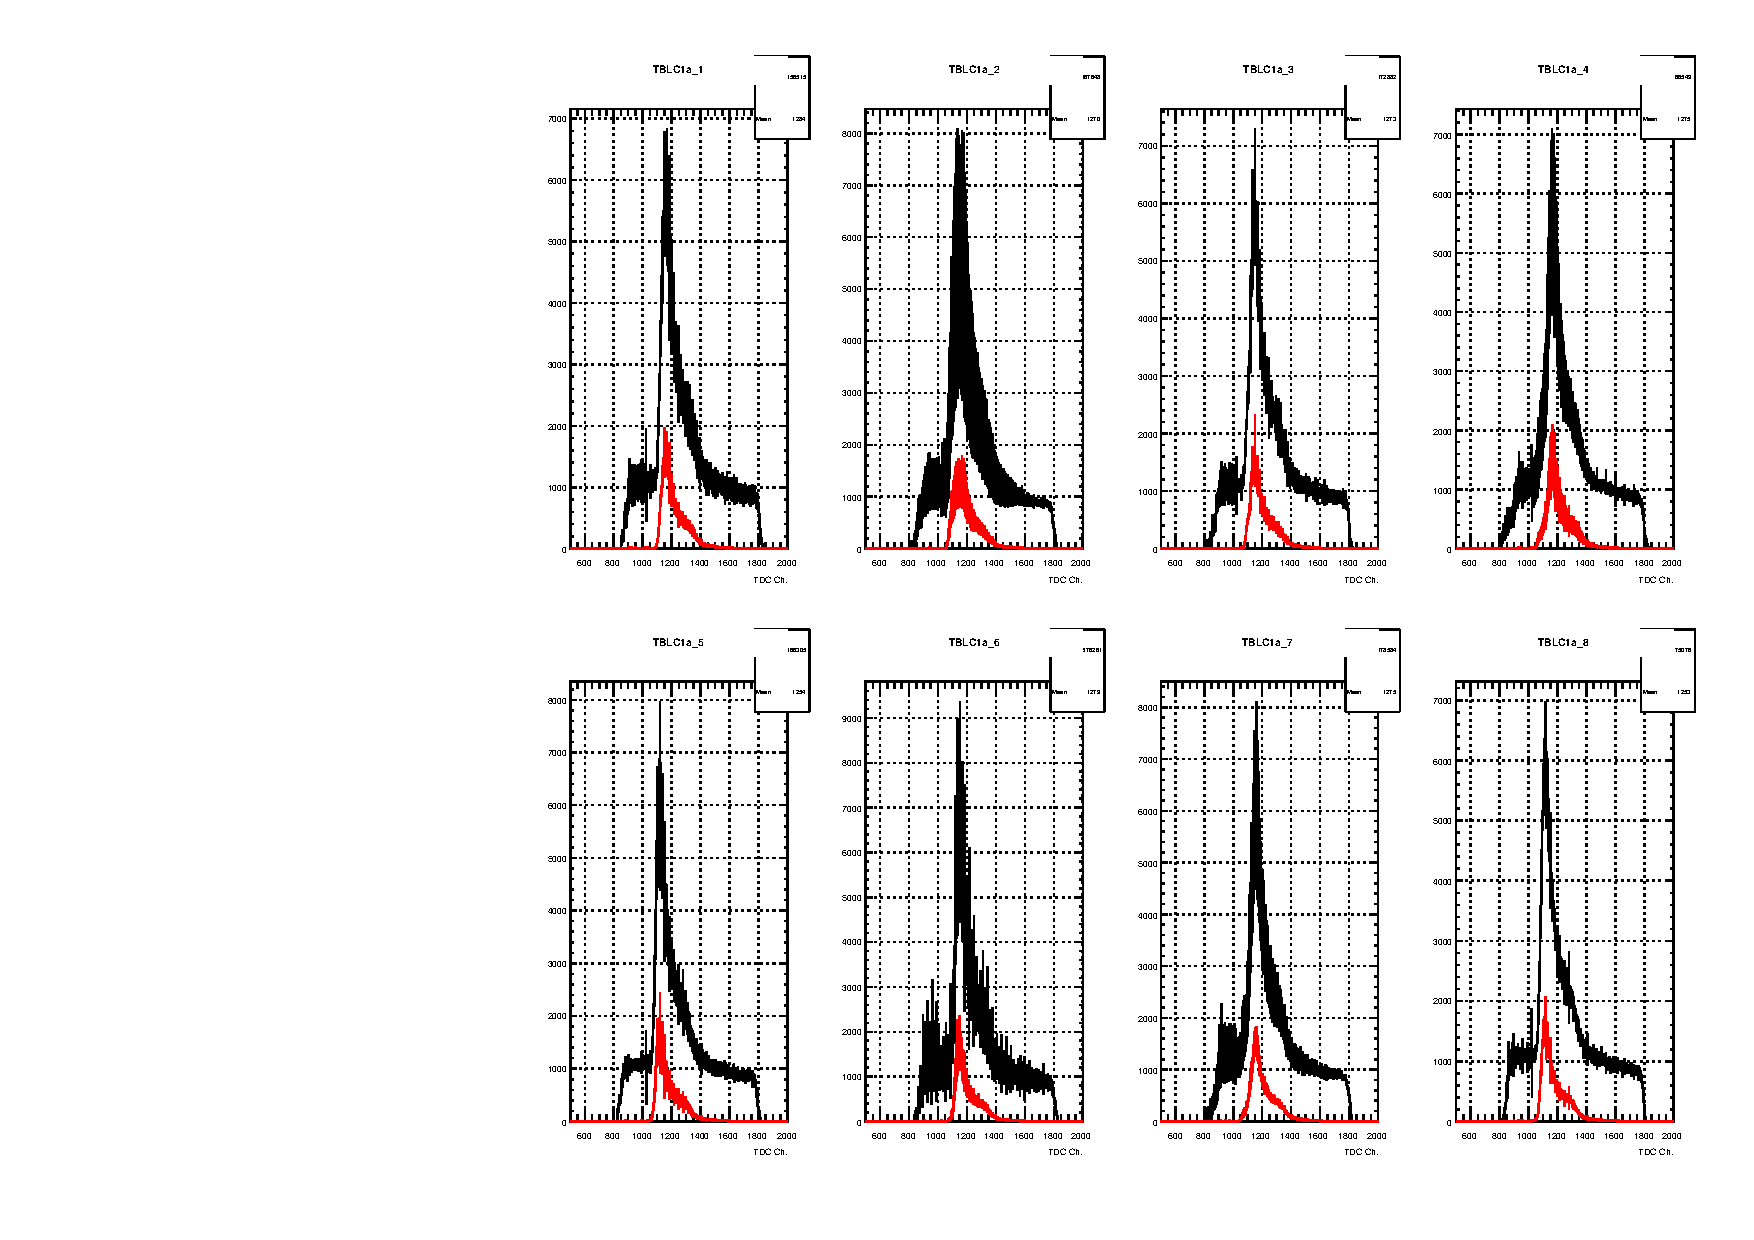
\includegraphics[width=0.95\linewidth]{TDCBLC1a}
\caption{TDC distribution of BLC1a. The black histogram shows a TDC distribution without any cuts. The red histogram shows a TDC distribution with a multiplicity cut (1 hit). }
\label{fig:TDCBLC1a}
\end{figure}

\begin{figure}
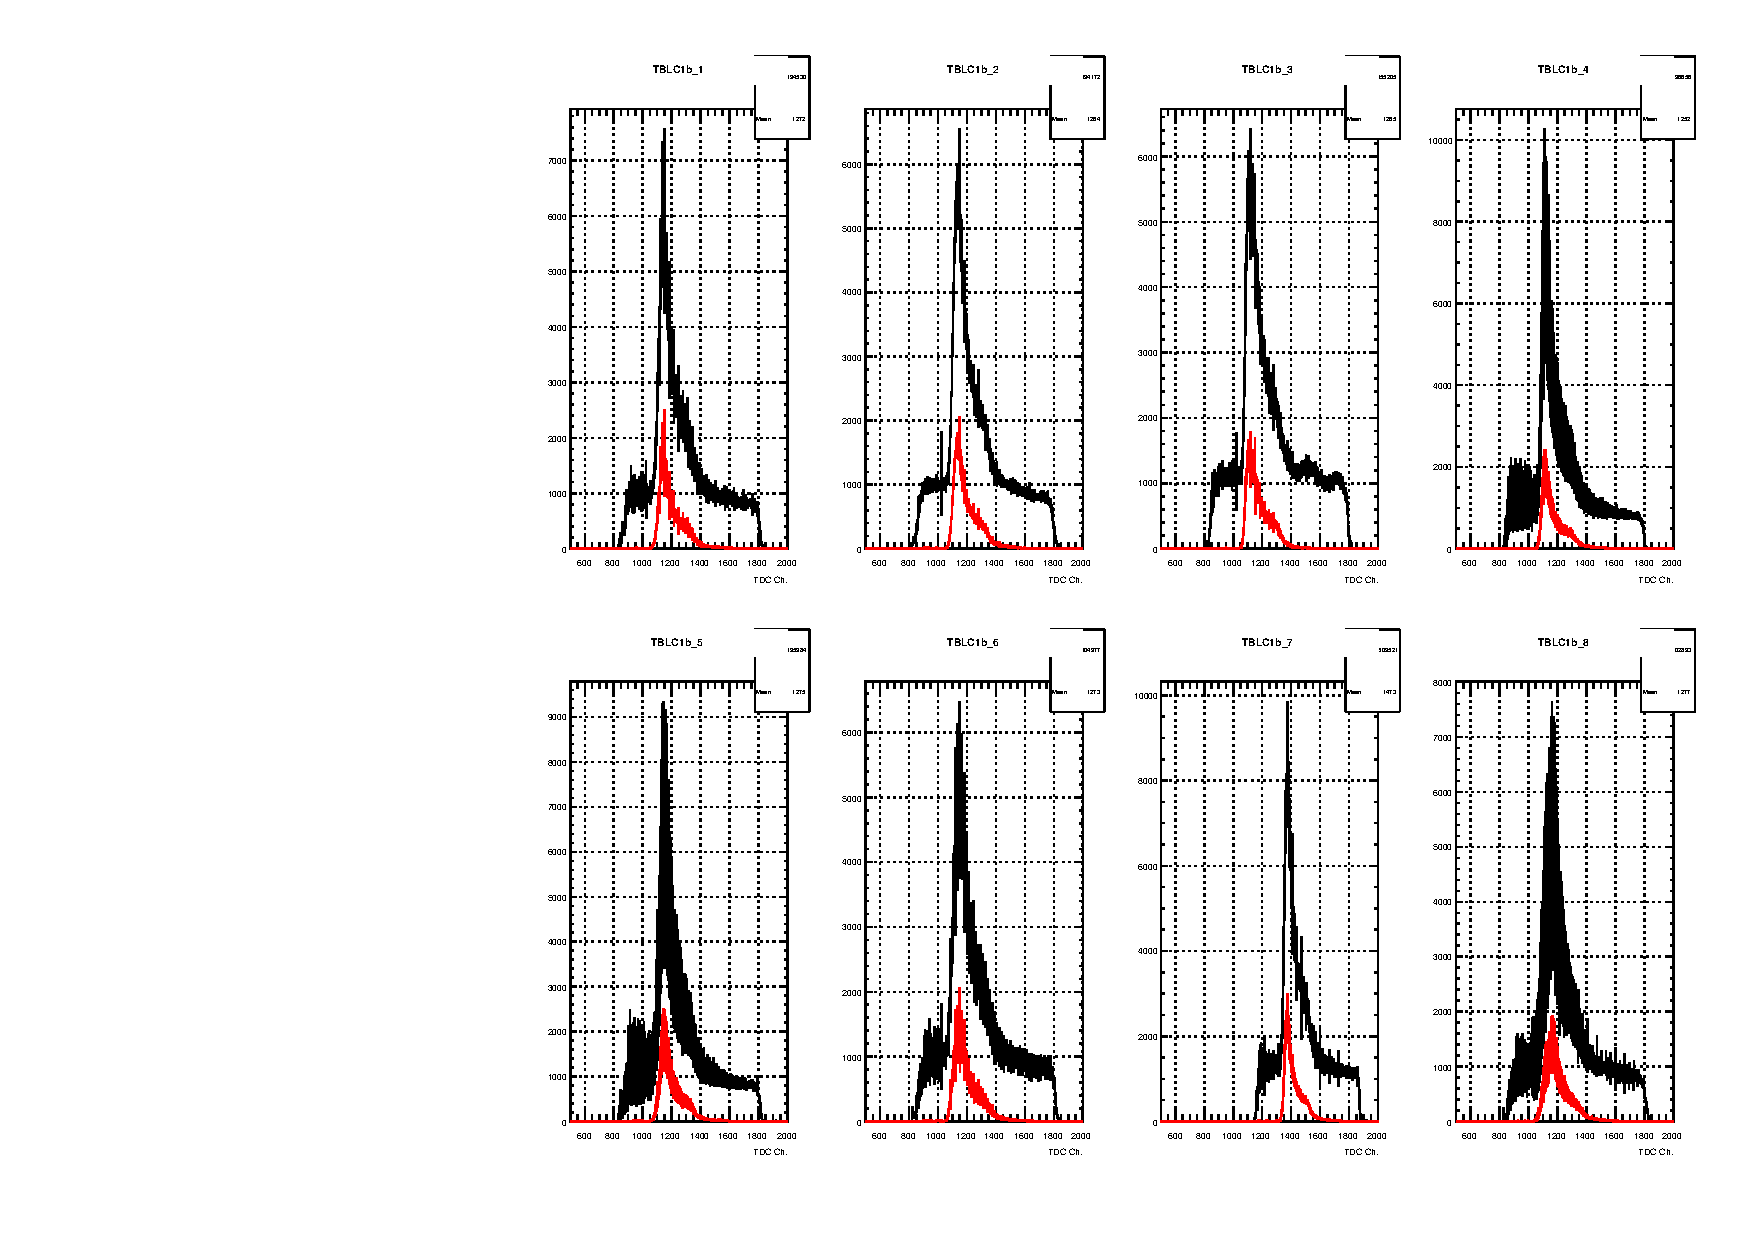
\includegraphics[width=0.95\linewidth]{TDCBLC1b}
\caption{TDC distribution of BLC1b, }
\label{fig:TDCBLC1b}
\end{figure}

\begin{figure}
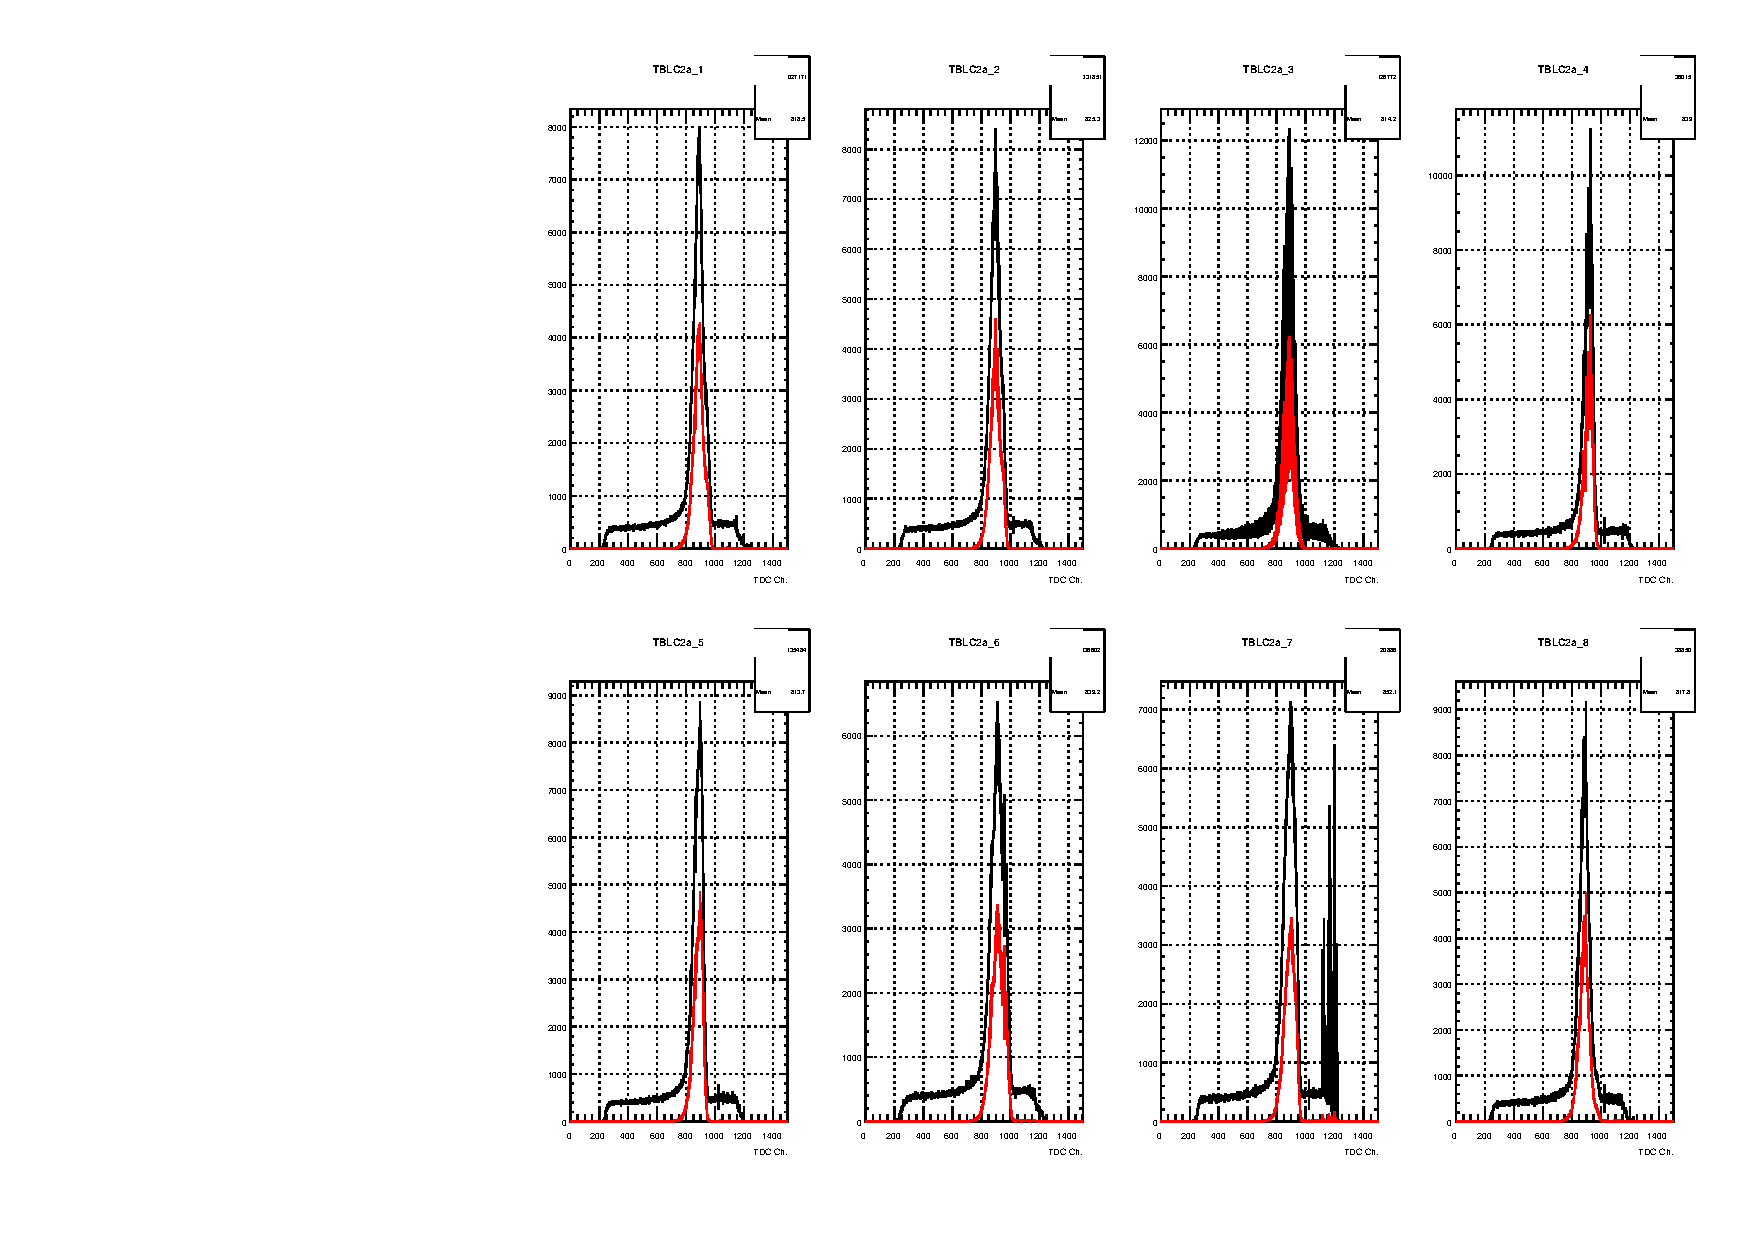
\includegraphics[width=0.95\linewidth]{TDCBLC2a}
\caption{TDC distribution of BLC2a, }
\label{fig:TDCBLC2a}
\end{figure}

\begin{figure}
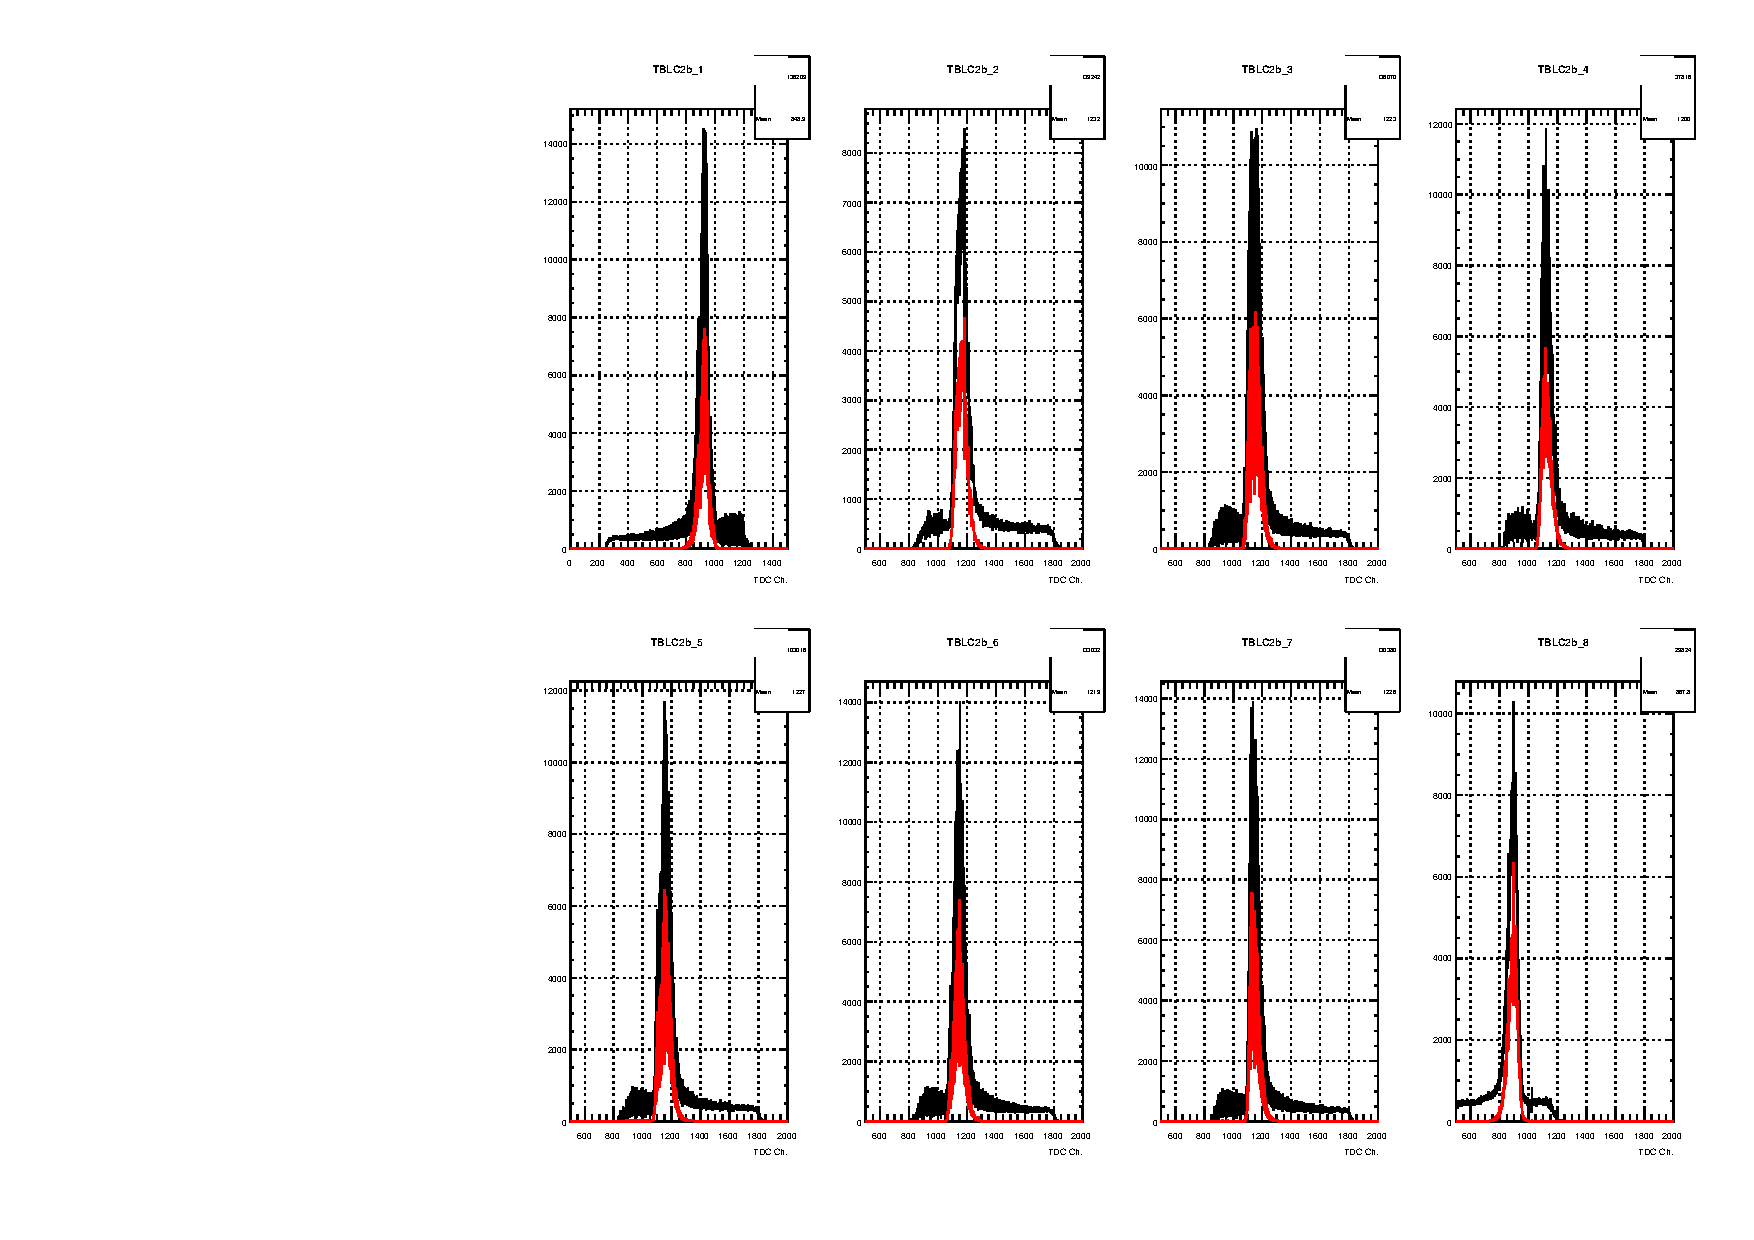
\includegraphics[width=0.95\linewidth]{TDCBLC2b}
\caption{TDC distribution of BLC2b, }
\label{fig:TDCBLC2b}
\end{figure}

\begin{figure}
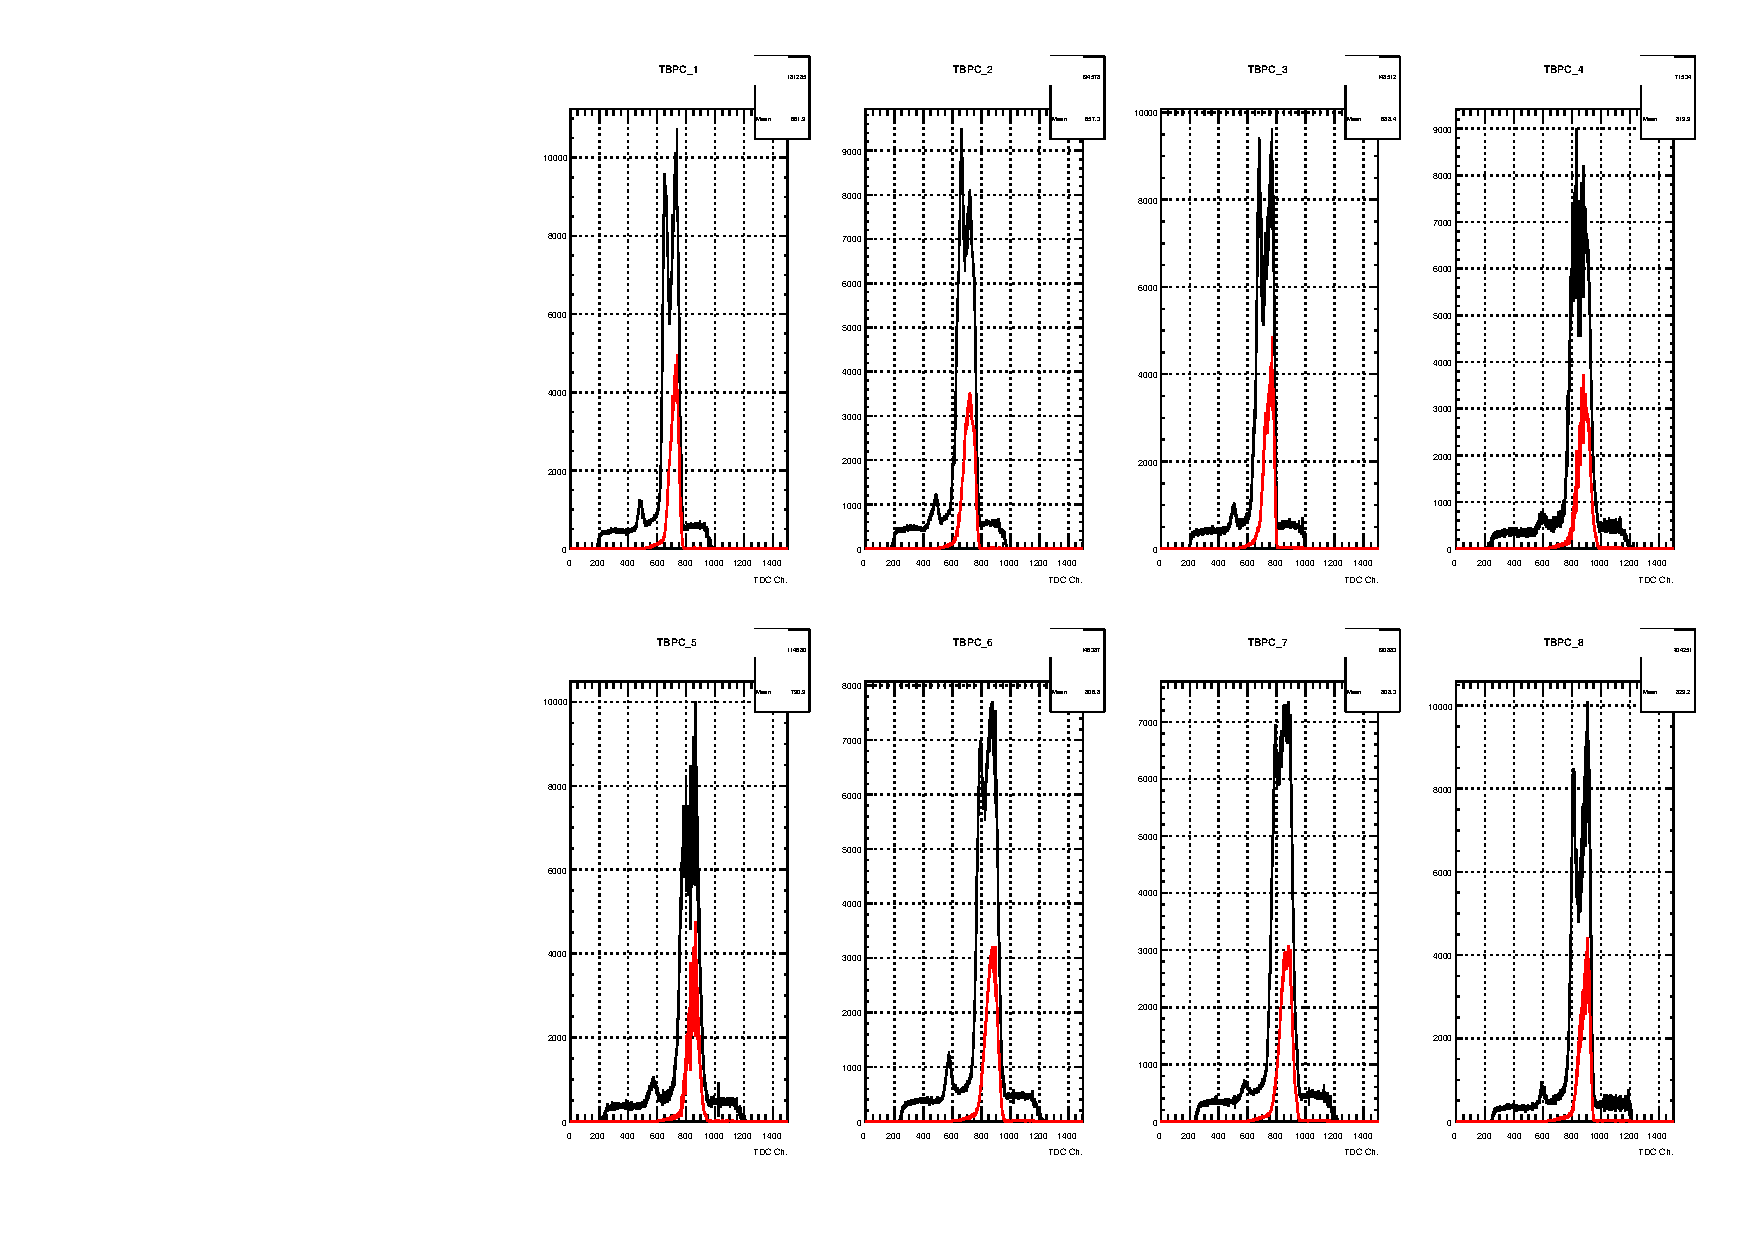
\includegraphics[width=0.95\linewidth]{TDCBPC}
\caption{TDC distribution of BPC, }
\label{fig:TDCBPC}
\end{figure}

\begin{figure}
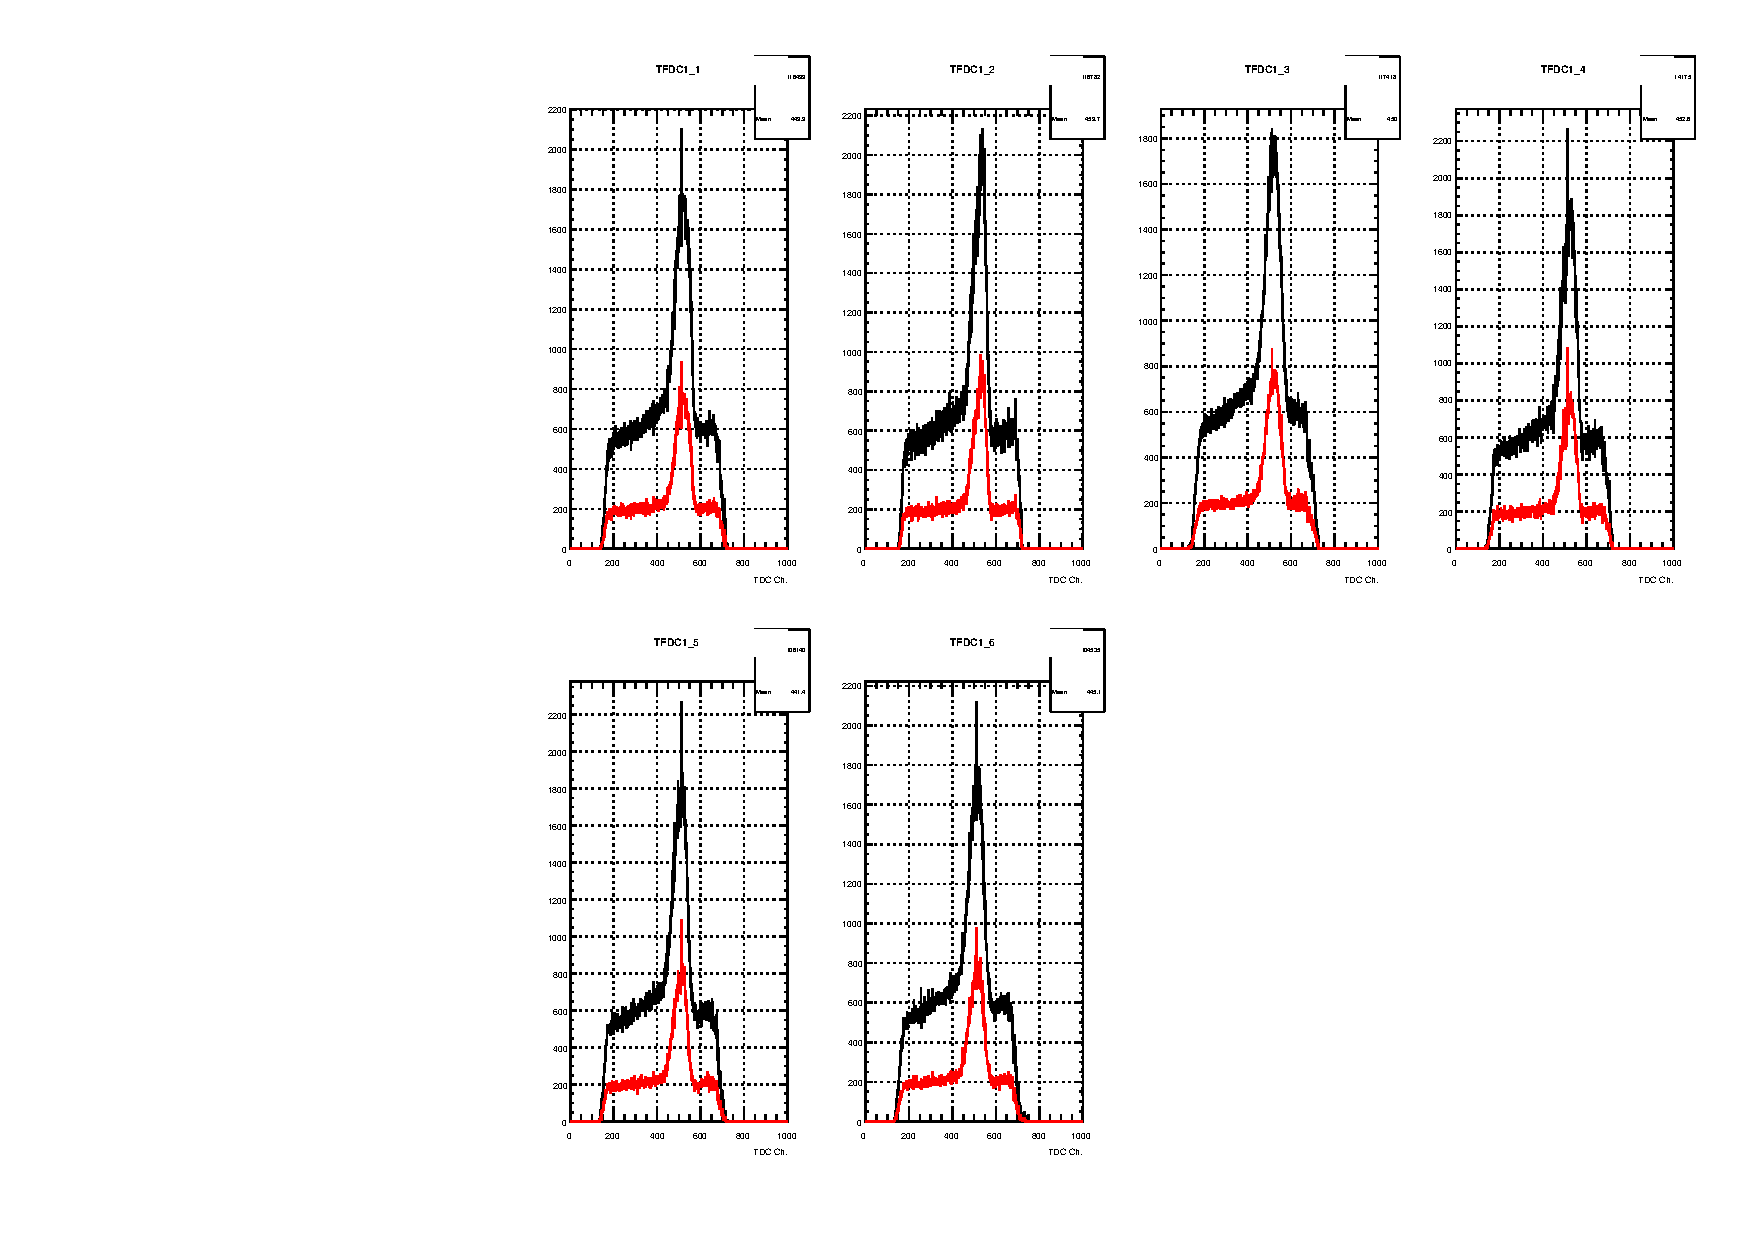
\includegraphics[width=0.95\linewidth]{TDCFDC1}
\caption{TDC distribution of FDC, }
\label{fig:TDCFDC1}
\end{figure}

\begin{figure}
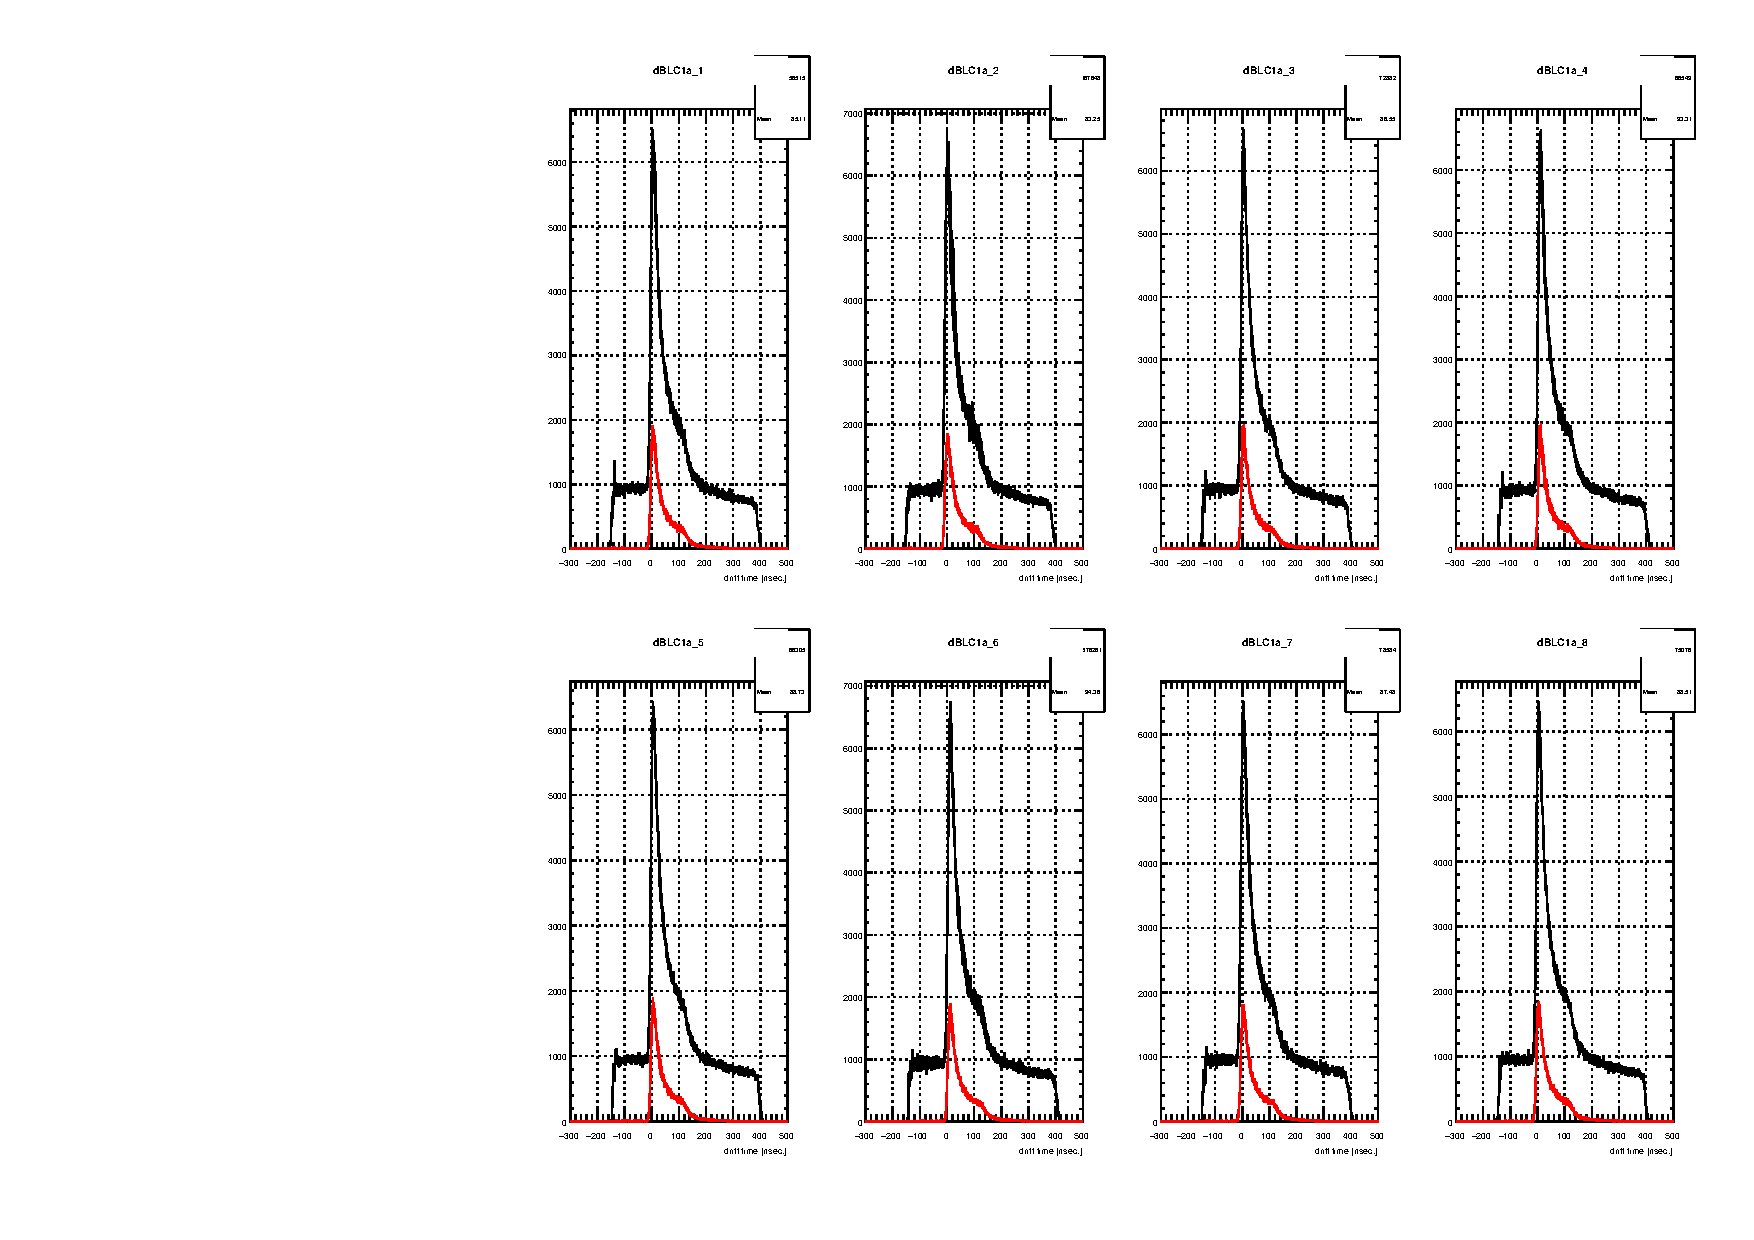
\includegraphics[width=0.95\linewidth]{dtBLC1a}
\caption{Drift time distribution of BLC1a, }
\label{fig:dtBLC1a}
\end{figure}

\begin{figure}
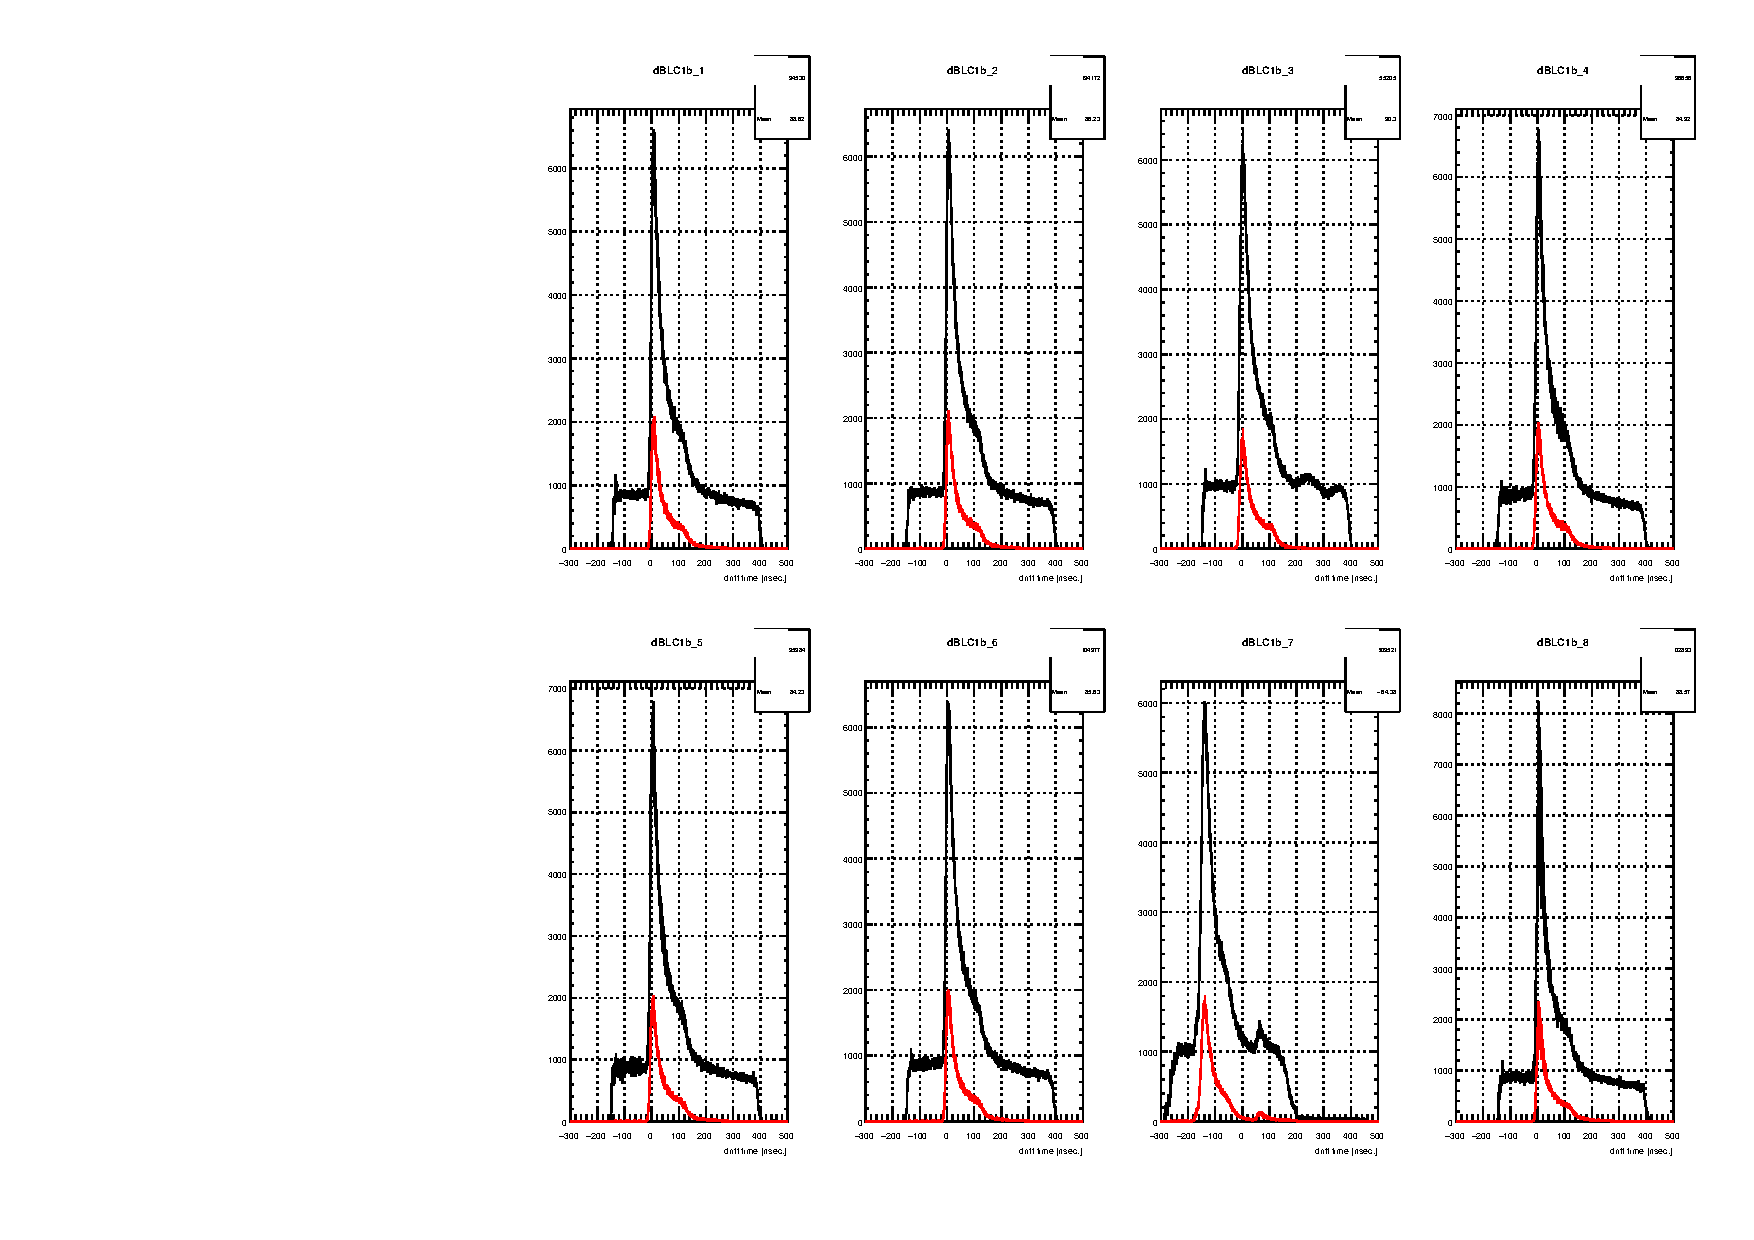
\includegraphics[width=0.95\linewidth]{dtBLC1b}
\caption{Drift time distribution of BLC1b, }
\label{fig:dtBLC1b}
\end{figure}

\begin{figure}
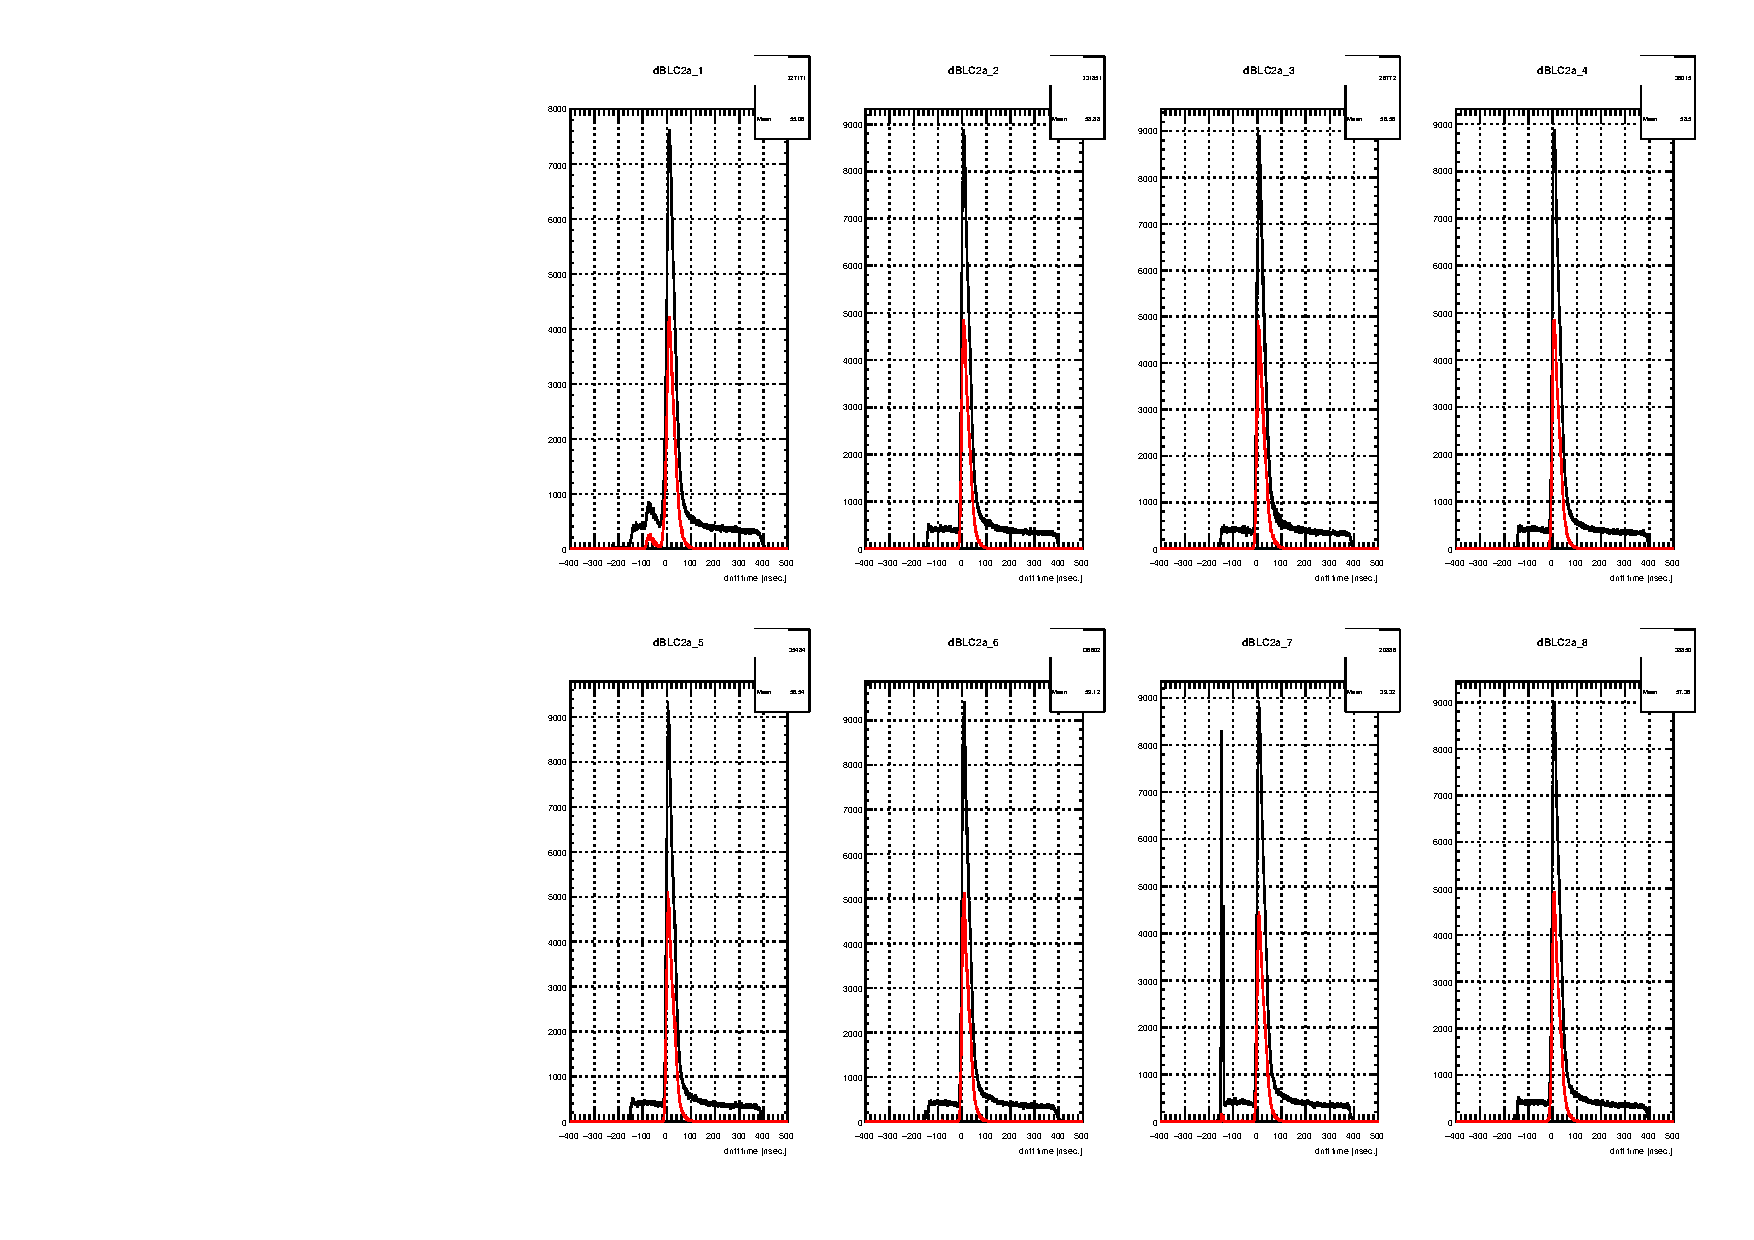
\includegraphics[width=0.95\linewidth]{dtBLC2a}
\caption{Drift time distribution of BLC2a, }
\label{fig:dtBLC2a}
\end{figure}

\begin{figure}
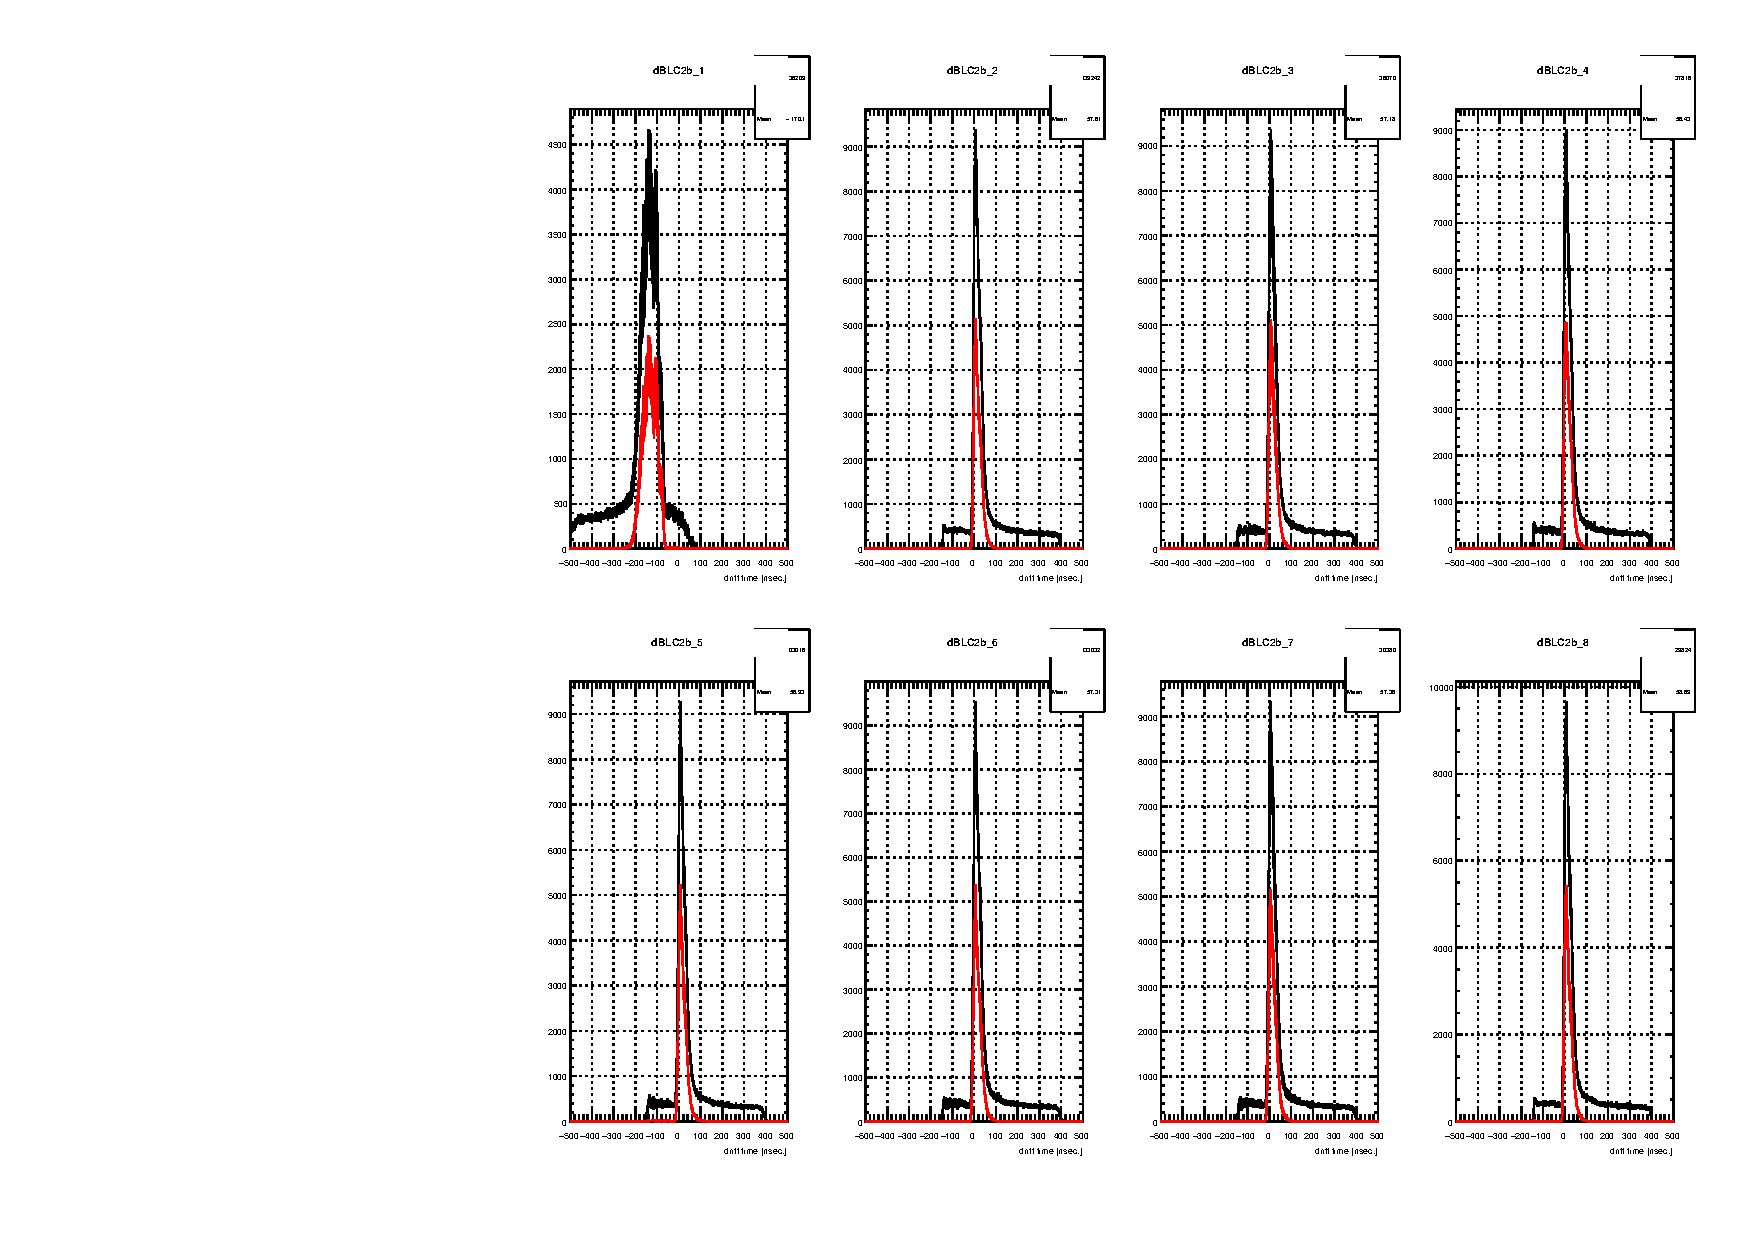
\includegraphics[width=0.95\linewidth]{dtBLC2b}
\caption{Drift time distribution of BLC2b, }
\label{fig:dtBLC2b}
\end{figure}

\begin{figure}
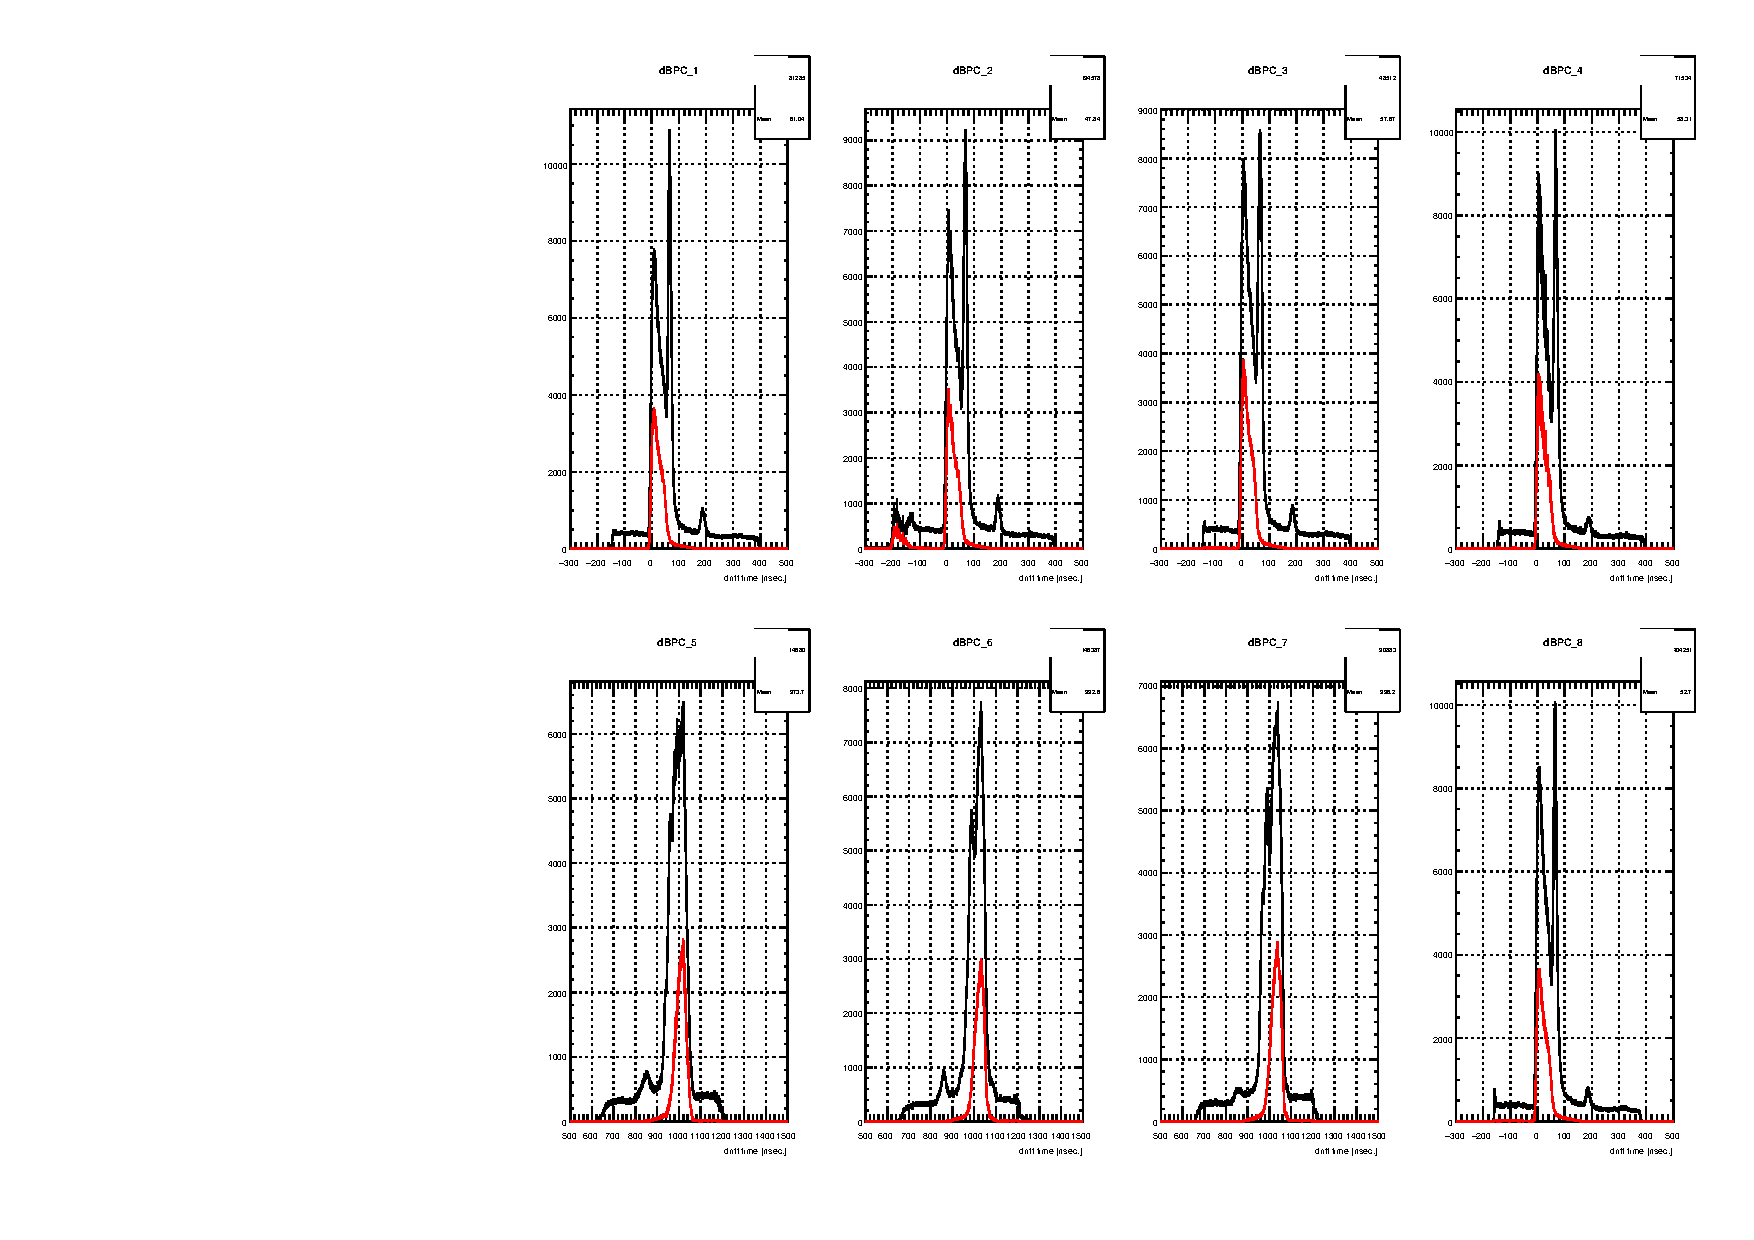
\includegraphics[width=0.95\linewidth]{dtBPC}
\caption{Drift time distribution of BPC, }
\label{fig:dtBPC}
\end{figure}

\begin{figure}
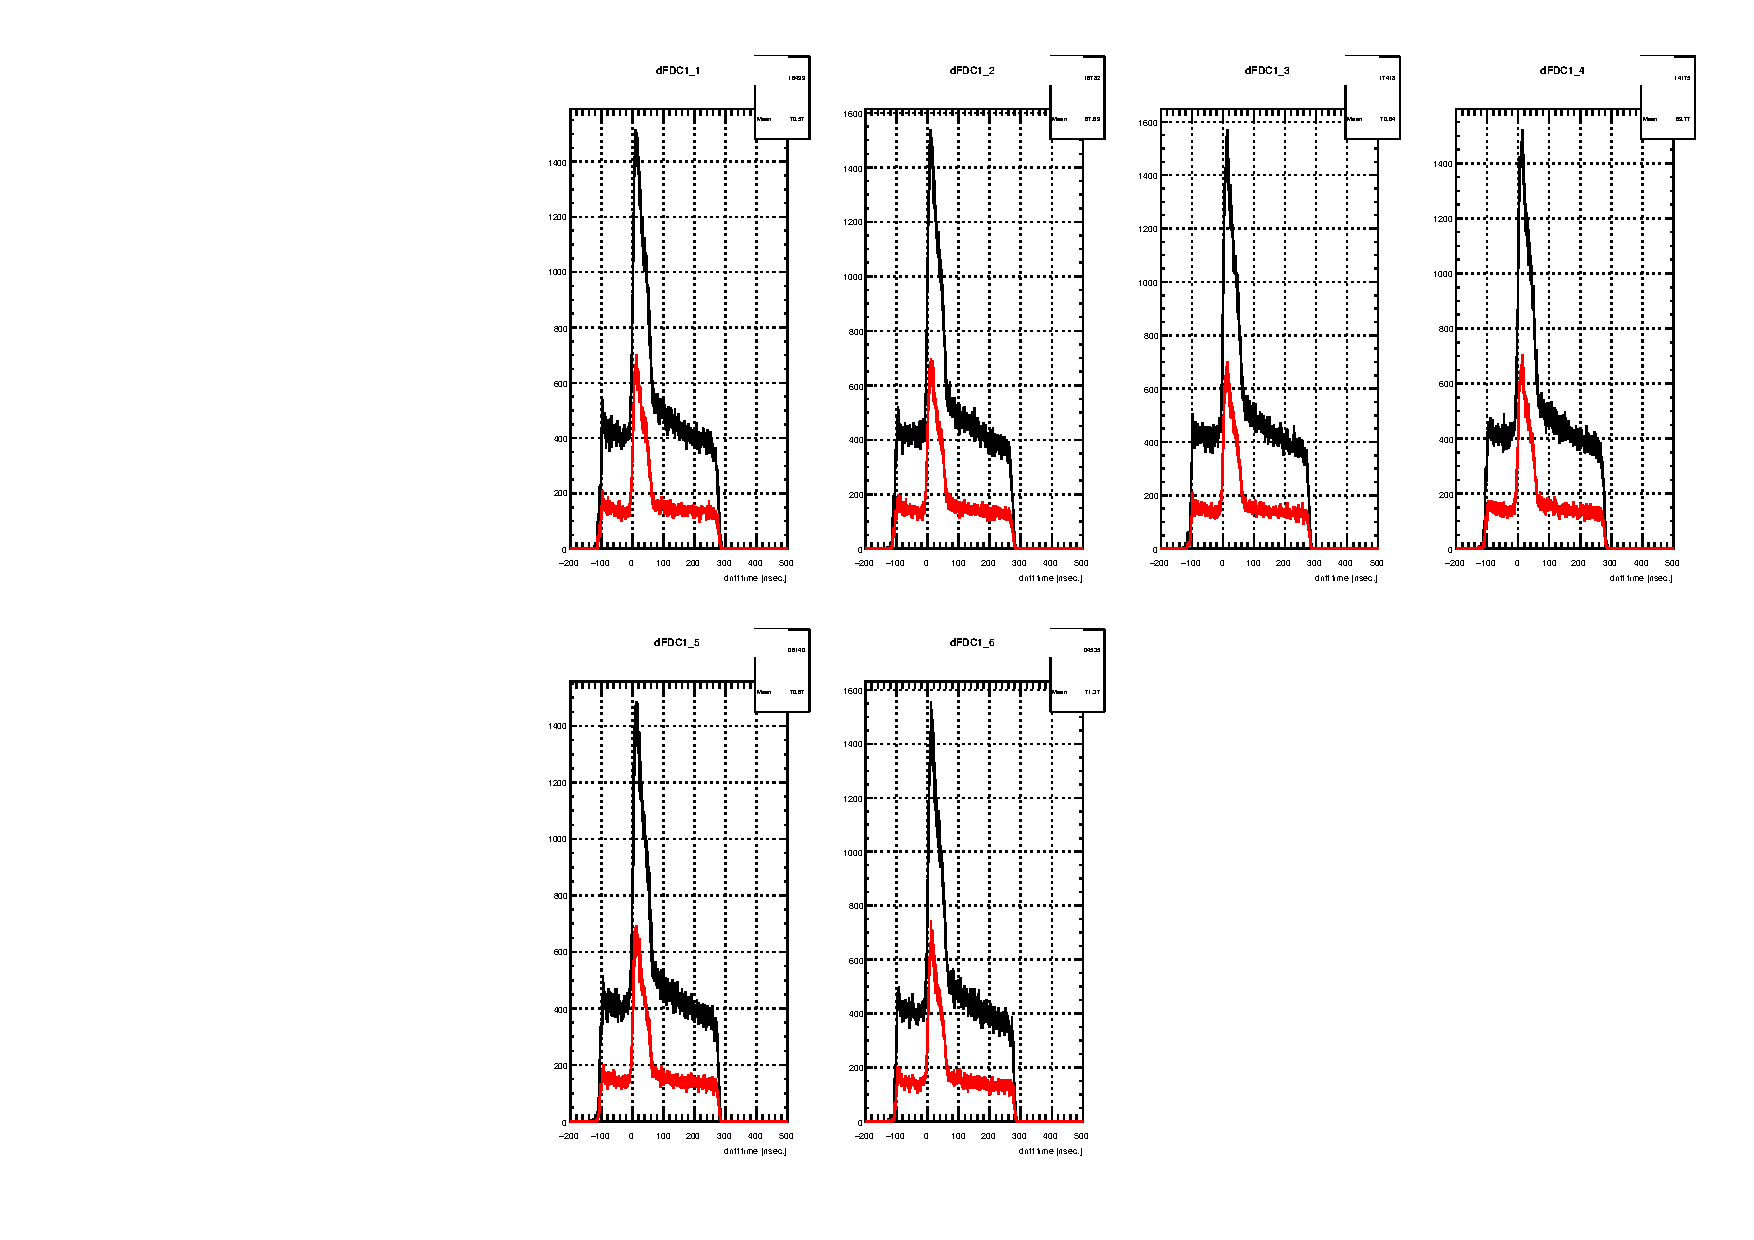
\includegraphics[width=0.95\linewidth]{dtFDC1}
\caption{Drift time distribution of FDC, }
\label{fig:dtFDC1}
\end{figure}




\subsubsection{CDC}

\subsection{Drift time correction by staggered wires}
To resolve left-right ambiguities, the planes of each pair are staggered by half of a cell size. There are correlation between a difference and a mean of drift time in the pair. By using the correlation, drift times can be improved.
In this analysis, clustering and tracking are performed.  It is required there are only 1 track in each drift chamber. The difference and the mean of drift time are extracted from the cluster made from hits in the staggered plane. 

\subsection{ADC calibration}

\subsection{Slewing Correction}

\subsection{Detector alignment}


\subsection{Target empty run}
